\documentclass[a4paper,11pt]{article}
\usepackage[utf8]{inputenc}
\usepackage[T1]{fontenc}
\usepackage[french]{babel}
\usepackage[right=2.3cm, left=2.3cm, bottom=3cm, top=2.2cm]{geometry}
\usepackage[ddmmyyyy]{datetime}
\usepackage[table]{xcolor}
\usepackage{lmodern,mathptmx,changepage,titlesec,hyperref,listings,lstautogobble,graphicx,array,longtable,multirow,lipsum,tikz,shorttoc,enumitem,float,verbatim, amsthm,amsmath,amssymb,mathrsfs,thmtools}
\usetikzlibrary{arrows,automata}
\usetikzlibrary{positioning}

\renewcommand{\rmdefault}{\sfdefault} %Utilisation de la police sans-serif ("Computer Modern Sans") pour la police roman
\renewcommand{\ttdefault}{pcr} 	%Utilisation d'une police "CourrierNew" pour la police monospaced (pour faire un listing manuel)
\linespread{1.15}				%Interligne

%Utilisation de liens colorés en bleu et soulignés
\hypersetup{colorlinks=true, urlcolor=blue, urlbordercolor=blue, linkcolor=black, linkbordercolor=white}
\makeatletter \Hy@AtBeginDocument{\def\@pdfborder{0 0 1} \def\@pdfborderstyle{/S/U/W 1}}\makeatother

\titlespacing*{\section} {0cm}{7ex plus 1ex minus .2ex}{1.5ex plus .2ex}
\titlespacing*{\subsection} {0cm}{4.5ex plus 1ex minus .2ex}{1.5ex plus .2ex}
\titleformat*{\section}{\LARGE\bfseries}
\titleformat*{\subsection}{\Large\bfseries}
\titleformat*{\subsubsection}{\normalsize\bfseries}

\definecolor{darkgreen}{rgb}{0,0.8,0}
\definecolor{mygray}{rgb}{0.93,0.93,0.93}
\definecolor{mymauve}{rgb}{0.58,0,0.82}
\lstset{	
	language=C,
	captionpos=b,
	basicstyle=\small\ttfamily,
	backgroundcolor=\color{mygray},
	breaklines=true,
	breakatwhitespace=true,
	tabsize=3,
	frame=none,
	rulecolor=\color{black},
	keywordstyle=\color{blue}\bfseries,
	stringstyle=\color{orange},
	showstringspaces=false,
	commentstyle=\footnotesize\color{darkgreen},
	keepspaces=true,
	extendedchars=true,
	numbers=left,
	numberstyle=\tiny\color{lightgray},
	stepnumber=1,
	escapeinside={(@}{@)},
	autogobble=true,
	literate=
		{á}{{\'a}}1 {é}{{\'e}}1 {í}{{}}1 {ó}{{\'o}}1 {ú}{{\'u}}1
		{Á}{{\'A}}1 {É}{{\'E}}1 {Í}{{\'I}}1 {Ó}{{\'O}}1 {Ú}{{\'U}}1
		{à}{{\`a}}1 {è}{{\`e}}1 {ì}{{\`i}}1 {ò}{{\`o}}1 {ù}{{\`u}}1
		{À}{{\`A}}1 {È}{{\'E}}1 {Ì}{{\`I}}1 {Ò}{{\`O}}1 {Ù}{{\`U}}1
		{ä}{{\"a}}1 {ë}{{\"e}}1 {ï}{{\"i}}1 {ö}{{\"o}}1 {ü}{{\"u}}1
		{Ä}{{\"A}}1 {Ë}{{\"E}}1 {Ï}{{\"I}}1 {Ö}{{\"O}}1 {Ü}{{\"U}}1
		{â}{{\^a}}1 {ê}{{\^e}}1 {î}{{\^i}}1 {ô}{{\^o}}1 {û}{{\^u}}1
		{Â}{{\^A}}1 {Ê}{{\^E}}1 {Î}{{\^I}}1 {Ô}{{\^O}}1 {Û}{{\^U}}1
		{œ}{{\oe}}1 {Œ}{{\OE}}1 {æ}{{\ae}}1 {Æ}{{\AE}}1 {ß}{{\ss}}1
		{ç}{{\c c}}1 {Ç}{{\c C}}1 {ø}{{\o}}1 {å}{{\r a}}1 {Å}{{\r A}}1
		{€}{{e}}1 {£}{{\pounds}}1 {«}{{\guillemotleft}}1
		{»}{{\guillemotright}}1 {ñ}{{\~n}}1 {Ñ}{{\~N}}1 {¿}{{?`}}1
}

%Redéfinition de la taille de \Huge pour le titre du document
\makeatletter\renewcommand\Huge{\@setfontsize\Huge{32pt}{40}}\makeatother
\date{\today}

%\usepackage[french,frenchkw,ruled,vlined]{algorithm2e}

\title{\vspace{\fill}\textbf{\Huge Contrôle continu}}
\author{
	Malek Zemni
	\vspace{2em}\\
	\textit{Attaque par faute sur DES}
	\vspace{2em}
}

\declaretheorem[name=Théorème]{Th}


\begin{document}
\pagenumbering{gobble}\clearpage
\maketitle\vspace{9em}
\begin{center}
\includegraphics[scale=0.7]{logo.png}\end{center}
\begin{flushright}Calcul sécurisé\end{flushright}

\newpage\clearpage\pagenumbering{arabic}

	
	\section*{Question 1 :} 
		
		\noindent Description d'une attaque par faute contre le DES sur la sortie $R_{15}$ du 15\up{ème} tour.
		
		\paragraph{} L'attaque par faute contre le DES est une attaque provoquant une faute intentionnelle dans l'algorithme afin de compromettre ses calculs. Cette faute va permettre de révéler une partie de la clé utilisée. Une attaque par recherche exhaustive sur la clé du DES a une complexité de $2^{56}$. L'objectif de l'attaque par faute est donc d'accélérer la recherche.
		
		\paragraph{} Dans notre cas, la faute est provoquée à la sortie $R_{15}$ du 15\up{ème} tour de Feitsel du DES. Il s'agit d'un échange d'un seul bit parmi les 32 bits de $R_{15}$ (\textit{single bit flip}), ce qui va donner une sortie fausse au 15\up{ème} tour qu'on note $R_{15}^{*}$. La figure ci-dessous illustre l'injection d'une faute à la sortie 15\up{ème} tour du DES :
		
		\begin{center}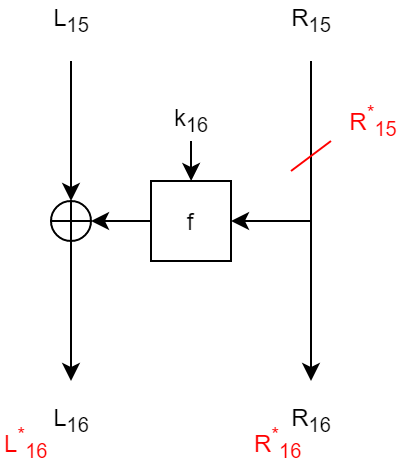
\includegraphics[scale=0.4]{DES_atq.png}\end{center}
		
		Pour exploiter cette faute, on va analyser les résultats obtenus à la sortie du 16\up{ème} tour. On a :
		\begin{itemize}
			\item $L_{16} = L_{15} \oplus f(R_{15}, k_{16})$
			\item $R_{16} = R_{15}$
			\item $L_{16}^{*} = L_{15} \oplus f(R_{15}^{*}, k_{16})$
			\item $L_{16}^{*} = R_{15}^{*}$
		\end{itemize}
		
		On remarque que $L_{16}$ et $L_{16}^{*}$ font toutes les deux intervenir la clé $k_{16}$ qui est l'objet initial de cette attaque. On exploite donc $L_{16}$ et $L_{16}^{*}$ pour construire une équation permettant de retrouver $k_{16}$. On effectue un XOR entre $L_{16}$ et $L_{16}^{*}$ pour éliminer $L_{15}$, l'équation obtenue est donc :
		\[L_{16} \oplus L_{16}^{*} = f(R_{15}, k_{16}) \oplus f(R_{15}^{*}, k_{16}) \]
		
		On va maintenant s'intéresser à la fonction interne $f$ du DES afin de mieux exploiter l'équation obtenue précédemment. Cette fonction est illustrée par la figure ci-dessous :
		
		\begin{center}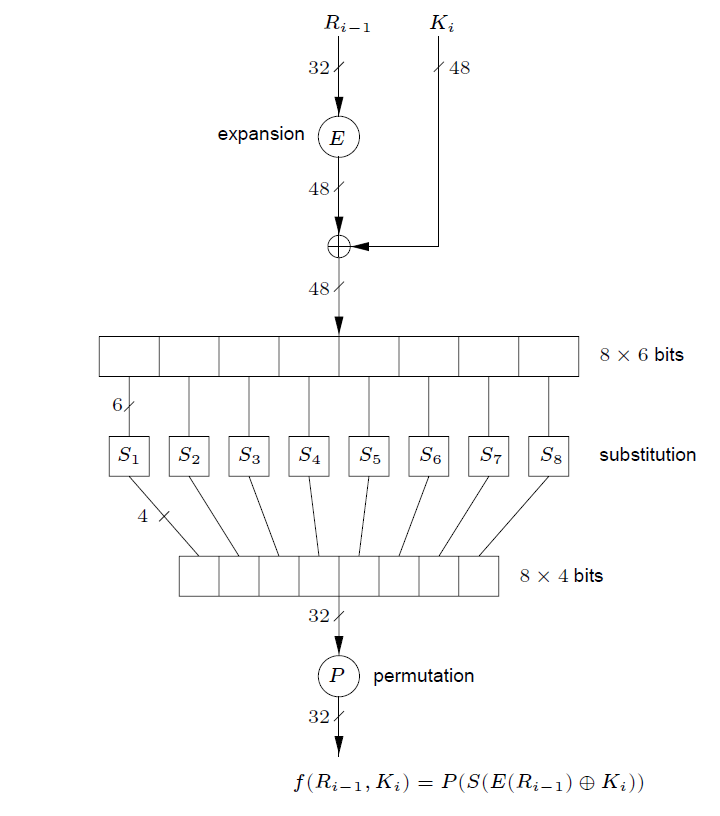
\includegraphics[scale=0.7]{DES_f.png}\end{center}
		
		L'analyse de cette fonction nous permet d'établir que :
		\begin{itemize}
			\item $f(R_{15}, k_{16}) \ = \ P\ [ \quad S_{1}({E(R_{15}) \oplus k_{16}}_{\ \textrm{bits}\ 1 \to 6}) \quad ||\ ...\ || \quad S_{8}({E(R_{15}) \oplus k_{16}}_{\ \textrm{bits}\ 43 \to 48}) \quad ]$			
			\item $f(R_{15}^{*}, k_{16}) \ = \ P\ [ \quad S_{1}({E(R_{15}^{*}) \oplus k_{16}}_{\ \textrm{bits}\ 1 \to 6}) \quad ||\ ...\ || \quad S_{8}({E(R_{15}^{*}) \oplus k_{16}}_{\ \textrm{bits}\ 43 \to 48}) \quad ]$
		\end{itemize}
		
		En effet, la fonction $f$ prend en entré le demi-bloc $R$ de 32 bits auquel elle applique une expansion de 48 bits, ainsi que la clé $k_{16}$. Ces deux entrées sont mélangées à l'aide d'un XOR pour obtenir une entité de 48 bits. Ces 48 bits vont être répartis sur 8 boites de substitution appelées \textit{S-box}. Chacune des 8 S-box prend 6 bits en entrée et en renvoie 4, pour avoir un résultat final de 32 bits. Ces S-box vont être l'objet principal de l'attaque. L'équation précédemment établie devient ainsi :
		\[L_{16} \oplus L_{16}^{*} = f(R_{15}, k_{16}) \oplus f(R_{15}^{*}, k_{16}) \]
		\[\Leftrightarrow\]		
		\[L_{16} \oplus L_{16}^{*}\]
		\[=\] 
		\[P\ [\ S_{1}({E(R_{15}) \oplus k_{16}}_{\ \textrm{bits}\ 1 \to 6}) \quad ||\ ...\ || \quad S_{8}({E(R_{15}) \oplus k_{16}}_{\ \textrm{bits}\ 43 \to 48})\ ] \]
		\[\oplus\] 
		\[P\ [\ S_{1}({E(R_{15}^{*}) \oplus k_{16}}_{\ \textrm{bits}\ 1 \to 6}) \quad ||\ ...\ || \quad S_{8}({E(R_{15}^{*}) \oplus k_{16}}_{\ \textrm{bits}\ 43 \to 48})\ ] \]
		
		\noindent En appliquant l'inverse de la permutation P (calculée à la main en prenant le chemin inverse de la permutation P fournie dans la documentation du DES), et en s'appuyant la propriété d'une permutation P quelconque, $P(a \oplus b) = P(a) \oplus P(b)$, on obtient :
		\[P^{-1}(L_{16} \oplus L_{16}^{*})\]
		\[=\] 
		\[ S_{1}\ ({E(R_{15}) \oplus k_{16}}_{\ \textrm{bits}\ 1 \to 6})\quad \oplus \quad S_{1}\ ({E(R_{15}^{*}) \oplus k_{16}}_{\ \textrm{bits}\ 1 \to 6}) \]
		\[||\ ...\ ||\]
		\[ S_{8}\ ({E(R_{15}) \oplus k_{16}}_{\ \textrm{bits}\ 43 \to 48})\quad \oplus \quad S_{8}\ ({E(R_{15}^{*}) \oplus k_{16}}_{\ \textrm{bits}\ 43 \to 48}) \]
		\\
		\noindent Finalement, en répartissant cette équation sur les 8 S-box, on obtient 8 équations dont les membres font 4 bits et les solutions font 6 bits :
		\begin{itemize}
			\item $P^{-1}(L_{16} \oplus L_{16}^{*})_{\ \textrm{bits}\ 1 \to 4}\ = \ S_{1}\ (E(R_{15}) \oplus k_{16})_{\ \textrm{bits}\ 1 \to 4}\ \oplus \ S_{1}\ (E(R_{15}^{*}) \oplus k_{16})_{\ \textrm{bits}\ 1 \to 4}$
			\item ...
			\item $P^{-1}(L_{16} \oplus L_{16}^{*})_{\ \textrm{bits}\ 29 \to 32}\ = \ S_{8}\ (E(R_{15}) \oplus k_{16})_{\ \textrm{bits}\ 29 \to 32}\ \oplus \ S_{8}\ (E(R_{15}^{*}) \oplus k_{16})_{\ \textrm{bits}\ 29 \to 32}$
		\end{itemize}
		
		La seule inconnue dans toutes ces équations est $k_{16}$. Pour trouver $k_{16}$, il faut faire une recherche exhaustive sur chacune des 8 S-box correspondant à chacune des 8 équations. Chaque recherche sur les S-box va permettre de révéler 6 bits de $k_{16}$, pour en avoir au final 48 bits. La complexité de cette attaque est donc de $8$ x $2^{6}$.
		
	\section*{Question 2 :}
		\subsection*{2.1 Recherche de la clé $k_{16}$ de 48 bits}
		\noindent \underline{Remarque} : les manipulations décrites dans cette partie sont implémentées dans le fichier source \lstinline!DES_K16.c!.
		
		\paragraph{} Dans la partie précédente, on est arrivé à établir 8 équations dont chacune révélait les 6 bits de $k_{16}$ qui rentrent dans chaque S-box. Cependant, il en faudrait plus qu'une simple recherche exhaustive sur chaque S-box, et ceci pour 2 raisons :
		
			\paragraph{Problème 1 : propagation du bit faux :}
				\paragraph{} Lors de l'attaque, la faute est introduite sur un seul bit parmi les 32 bits du demi-bloc sortant du 15\up{ème} tour du DES, $R_{15}$ qui devient $R_{15}^{*}$. Le problème est qu'un bit erroné n'agit pas sur toutes les 8 S-box que l'on va attaquer puisque les données entrantes aux S-box sont réparties par 6 bits.\\
				En effet, pour une S-box $i$ et des données de 6 bits allant de $x$ à $y$) :
				\[
				P^{-1}(L_{16} \oplus L_{16}^{*})_{\ \textrm{bits}\ x \to y}\ = \ S_{i}\ (E(R_{15}) \oplus k_{16})_{\ \textrm{bits}\ x \to y}\ \oplus \ S_{i}\ (E(R_{15}^{*}) \oplus k_{16})_{\ \textrm{bits}\ x \to y}
				\]
				Le problème survient lorsque sur ces 6 bits allant de $x$ à $y$, le bit erroné par l'attaque n'est pas propagé. Dans ce cas on aura $R_{15}\ =\ R_{15}^{*}$, ce qui induit aussi que $L_{16}\ =\ L_{16}^{*}$. L'équation qui permet la recherche sur cette S-box $i$ sera de la forme $0\ =\ 0$ ce qui ne révèlerait aucune information sur les 6 bits de $k_{16}$ allant de $x$ à $y$.
				
				\paragraph{} La solution pour remédier à ce problème est d'attaquer le DES par plusieurs fautes dont les bits erronés vont nécessairement se propager jusqu'au 6 bits en entrée de chacune des 8 S-box. En effet, pour assurer cela, il faut vérifier la table d'expansion des bits E :

				\begin{center}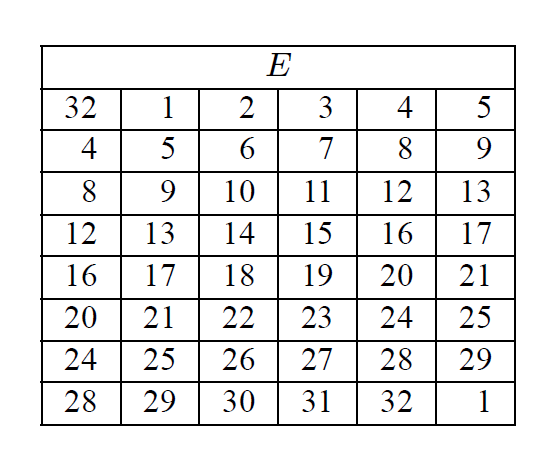
\includegraphics[scale=0.5]{E.png}\end{center}
				
				Cette table est utilisée pour effectuer une expansion de 32 bits du demi-bloc pris en entrée, en une entité de 48 bits. Ces 48 bits vont être découpées en 8 blocs de 6 bits. Par exemple une faute sur le 32\up{ème} bit va être propagée au 1\up{er} et 47\up{ème} bit de la sortie de l'expansion, et va ainsi se propager à la S-box 1 et 8. Donc pour une faute, on peut avoir une propagation sur une ou deux S-box au plus.
				
			\paragraph{Problème 2 : nombre de solutions des S-box :}
				\paragraph{} Une équation du type $y = S-box(x)$ peut avoir plusieurs solutions pour $x$, à cause de la manière dont une S-box est construite. De ce fait, une recherche exhaustive sur une S-box donnera potentiellement plusieurs solutions pour le 6 bits de $k_{16}$. Il est donc impossible de conclure quant aux bons 6 bits de $k_{16}$.
				
				\paragraph{} La solution pour remédier à ce problème est d'attaquer chaque S-box par plusieurs fautes. Pour chaque faute, on va faire une recherche exhaustive des solutions de la S-box concernée, tout en sauvegardant cet ensemble de solutions. La bonne solution qui sera prise en compte pour les 6 bit de $k_{16}$ est celle qui est en commun à toutes les fautes injectées.\\
				Il faut bien entendu préciser que les fautes utilisées pour attaquer chaque S-box doivent avoir des bits erronés qui se propagent bien sur les 8 S-box.
				
				
			\paragraph{Recherche $k_{16}$ :}
			
			\paragraph{} Compte tenu des problèmes énoncés, on peut maintenant procéder à la recherche de $k_{16}$.
			\begin{itemize}
				\item On commence d'abord par récupérer les 32 chiffrés faux fournis. Après analyse de ces chiffrés, on a pu récupérer pour chaque S-box 6 chiffrés faux dont on s'est assuré que le bit erroné va bien se propager dans la S-box concernée lors de la recherche exhaustive. Pour chacune des 8 S-box, on indique dans une table la position de ces 6 chiffrés faux :
				\lstinputlisting[caption={DES\_K16.c}, firstline=24, lastline=33]{../../App/src/DES_K16.c}
			
				\item Ensuite, on calcule les éléments vrais de l'équation ($R_{15}$ et $L_{16}$) :
				\lstinputlisting[caption={DES\_K16.c}, firstline=35, lastline=38]{../../App/src/DES_K16.c}
			
				\item On attaque maintenant attaque chacune de 8 S-box par 6 fautes, tout en recalculant à chaque fois les éléments faux de l'équation ($R_{15}^{*}$ et $L_{16}^{*}$) :
				\lstinputlisting[caption={DES\_K16.c}, firstline=41, lastline=79]{../../App/src/DES_K16.c}
				
				\item L'attaque va donner un ensemble de solutions possibles pour chacune des 6 fautes. Il faudra finalement récupérer la solution unique qui correspond aux bons 6 bits de $k_{16}$, et ceci pour chacune des 8 S-box :
				\lstinputlisting[caption={DES\_K16.c}, firstline=91, lastline=114]{../../App/src/DES_K16.c}
			\end{itemize}
			
			Voici un aperçu des différentes étapes de l'exécution de cette recherche de $k_{16}$ :
			
			\begin{center}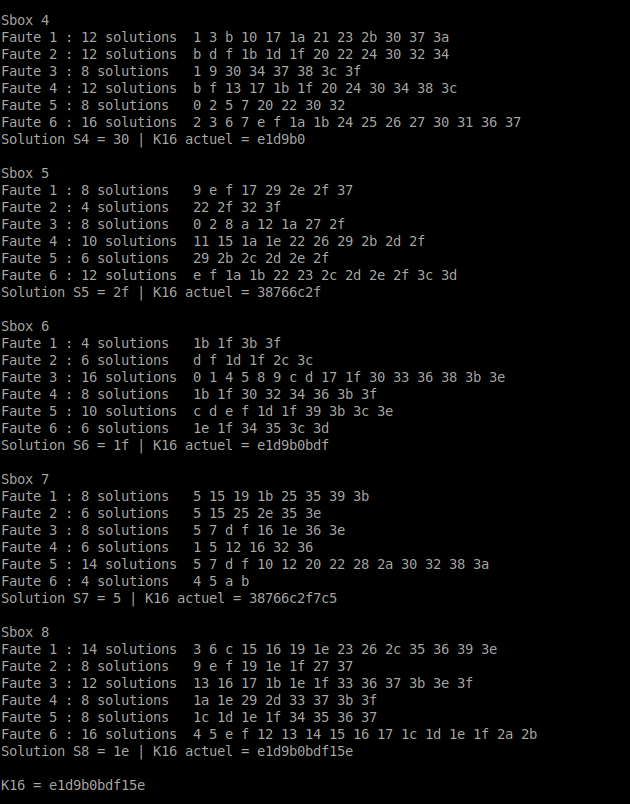
\includegraphics[scale=0.8]{K16.png}\end{center}
			
		\subsection*{2.2 Valeur de la clé $k_{16}$ de 48 bits}
		\[ \textrm{E1D9B0BDF15E} \]
		
	\section*{Question 3 :}
		
		\noindent \underline{Remarque} : les manipulations décrites dans cette partie sont implémentées dans le fichier source \lstinline!DES_K.c!.
		
		\subsection*{3.1 Recherche des 8 bits manquants}
			On a obtenu précédemment une clé $k_{16}$ de 48 bits. On va utiliser cette clé pour reconstituer la clé mère K de 64 bits. Pour cela, on va analyser l'algorithme de dérivation de clés qui est illustré dans la figure ci-dessous :
			\begin{center}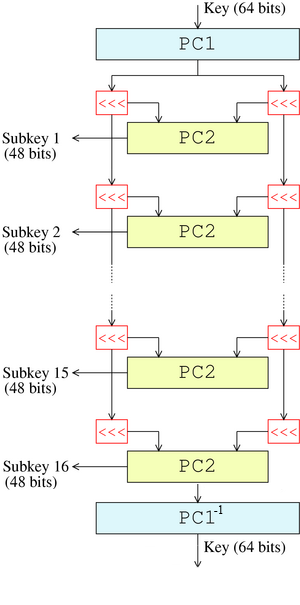
\includegraphics[scale=0.5]{KEY.png}\end{center}
			
			On remarque qu'en appliquant les inverses des 2 fonctions de permutation PC1 et PC2 à partir de $k_{16}$, on retombe sur la clé K de 64 bits. En effet,
			\[K\ =\ PC1^{-1}(\ PC2^{-1}(\ k_{16}\ ))\]
			
			Cependant, un problème se pose à cause de la nature de la permutation PC2. En effet, PC2 est une permutation qui prend 56 bits en entrée et en renvoie 48. Quand on applique la permutation inverse PC2\up{-1}, on prend 48 bits en entrée et on en renvoie 56. On perd les informations de 8 bits.\\
			\indent Ces 8 bits perdus ont des positions bien précises qu'on trouve par analyse de la permutation appliquer par PC2. Ces positions celles des bits 9, 18, 22, 25, 35, 38, 43 et 54. Lorsqu'on reconstruit la table de la permutation inverse PC2\up{-1}, on met la permutation à 0 pour ces positions.
			
			\paragraph{Recherche :} 
			\paragraph{} La première étape de la recherche des 8 bits perdus était de reconstituer une clé qu'on va appeler $K^{*}$ de 64 bits telle que $K^{*}\ =\ PC1^{-1}(\ PC2^{-1}(\ k_{16}\ ))$.\\
			\indent Ensuite, une fois qu'on a récupéré les positions bits perdus par PC2\up{-1} (9, 18, 22, 25, 35, 38, 43 et 54), on effectue une recherche exhaustive pour ces 8 bits (complexité au pire de $2^{8}$). Cette recherche va appliquer un masque différent sur la clé à chaque itération pour alterner les 8 bits aux positions précises sur les 64 bits de $K^{*}$ :
			\lstinputlisting[caption={DES\_K.c}, firstline=32, lastline=43]{../../App/src/DES_K.c}
			\lstinputlisting[caption={DES\_K.c}, firstline=9, lastline=18]{../../App/src/DES_K.c}
			
			\paragraph{Bits de parité :} 
			\paragraph{} La recherche des 8 bits perdus a permis de retrouver 56 bits parmi les 64 bits de la clé mère K. Les 8 bits qui restent sont les bits de parités. Ils n'interviennent pas dans l'opération de chiffrement du DES et n'ont donc pas d'impact lors de la recherche des 8 bits perdus.
			
			\paragraph{} Voici un aperçu des différentes étapes de l'exécution de la reconstitution de la clé mère K de 64 bits :
			
			\begin{center}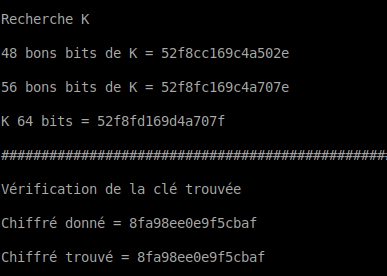
\includegraphics[scale=1]{K.png}\end{center}
			
		\subsection*{3.2 Valeur de la clé K de 64 bits}
		\[ \textrm{52F8FD169D4A707F} \]
			
\end{document}
